\chapter{Conclusion}%
\label{sec:conclusion}

To conclude this thesis,
 we should return to our
 original goal of
 supporting the thesis statement
 stated in \autoref{sec:intro}:
\begin{quote}
  \it\Thesisstmt
\end{quote}
There are a few important parts of this statement,
 and teasing them apart
 may help us figure out if
 we have done what we set out to do.

First, we start out with
 ``e-graphs and equality saturation \emph{are} compelling techniques [\ldots]''.
This introductory phrase deserves to stand alone.
Both the core technique discussed in this thesis
 and the data structure that powers it
 are exciting, well-developed prior work.
My hope is that the document as a whole---and the
 background in \autoref{sec:background} in
 particular---get this point across to the reader.
In the course of advancing the state-of-the-art
 in these areas,
 it is necessary to focus on their shortcomings,
 but hopefully this phrase expresses
 how just how tall these shoulders are.
Had I not been excited by these works,
 this thesis would not exist.

Second, we have
 ``e-graphs and equality saturation [\ldots] should \emph{now} be considered [\ldots]''.
This is not to say that they are not without merit on their own,
 but rather that I hope the advances introduced in this thesis
 help raise the profile of \eqsat as a compelling technique.
Chapters \ref{sec:rebuilding} and \ref{sec:extensions}
 present new approaches that makes \eqsat faster and more flexible,
 alleviating two key concerns with that a prospective user may have.
\autoref{sec:egg} introduces \egg,
 the tool that implements all of this
 and make \eqsat easier to use than ever before.
Put together, I believe these contributions make \emph{now}
 the time to look into and use \eqsat.

Finally, we end by stating that \eqsat should be applicable to
 ``[\ldots] programming tools across many domains.''
My goal for this thesis is to turn
 many ``why'' questions about equality saturation into ``why not'' questions.
The case studies in \autoref{sec:case-studies}
 hopefully offer empirical evidence that
 \eqsat can be useful (and even critical)
 in unexpected ways.
If the same technique can shrink 3D CAD programs (\autoref{sec:szalinski}),
 make floating point more accurate (\autoref{sec:herbie}),
 optimize deep learning compute graphs (\autoref{sec:tensat}),
 and synthesize the very rules that it needs to work (\autoref{sec:ruler}),
 then why wouldn't it work for your problem in your domain?
Even outside of those case studies,
 \egg is powering or inspiring many additional projects,
 only some of which are published at the time of writing
 this~\cite{spores, Cheli2021, diospyros}.


People used and worked on equality saturation before
 I began work on this thesis.
In fact,
 I first learned about it by
 talking to some of those people (the Herbie developers, \autoref{sec:herbie}).
My first reaction
 to equality saturation was that of a skeptic (``it's just unionfind''),
 and I began
 work on \egg out of hubris to show that it was trivial to implement.
Predictably, I was quickly humbled,
 but eventually \egg became a useful tool.
After some more learning,
 I moved into the fanatic phase: ``why isn't everyone doing this?''
Through the course of pushing a round \egg through several square holes,
 I would like to think that I have adopted a more pragmatic approach,\footnote{
   Friends and colleagues, however, will be excused for still thinking
   me a fanatic. 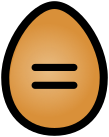
\includegraphics[height=1em]{egg.png}
}
 informed by the strengths and weaknesses of the technique.

This work in this thesis puts a dent in those weaknesses
 and introduces some new strengths.
With these advances,
 and with \egg packaging them all up,
 I hope that others find that equality saturation
 is a viable, useful, and even fun
 technique with a more straightforward journey than my own.

\section{Future Work}

Going forward,
 I hope and expect that equality saturation will
 take a larger role is all kinds
 of compilers, synthesizers, and optimizers.
But further work is needed to get there.
While \egg can already be used to build
 a state-of-the-art optimizer
 fast enough to use in a compiler~\cite{tensat},
 this only applies for domains
 with algebraic, context-free interpretations of their expressions.
To make \eqsat practical in more complex domains
 (like general purpose programming languages),
 new conceptual advances are required.

Prior work~\cite{eqsat} introduced
 \textit{Program Expression Graphs} (PEGs)
 to represent programs with mutation and loops inside \egraphs,
 but not
% While this allows representation of
%  low-level IRs like LLVM,
%  it does not solve the problem for
 source-level programs or functional IRs.
These latter two are tricky for \egraphs because binding means
 that equivalence is \textit{contextual}:
 two variables $x$ in the program might refer to different binding sites.
\Eclass analyses could be combined
 with recent work~\cite{hashing-alpha} that
 proposes a modular way to describe binding structure.

Complex domains will require larger search spaces,
 further pushing the performance requirements for \egraphs and \eqsat.
This work introduced a new, more efficient
 algorithm for congruence closure in \egraphs;
 the remaining bottleneck is
 e-matching.
\egg uses the current state-of-the-art~\cite{ematching}
 backtracking algorithm that wastes work when
 search for patterns like $(x * y) + (x * z)$ with multiple
 occurrences of the same variables.
A smarter e-matching algorithm could
 take advantage of these equality constraints,
 similar to how joins in a relational database do.

Finally, \eqsat's performance and correctness
 both hinge on the rewrites provided by the users.
If those rewrites are incomplete or unsound,
 \eqsat may miss optimizations or yield incorrect results.
Automatically generating these rules could make using \eqsat even
 easier for prospective users.

%%% Local Variables:
%%% TeX-master: "../thesis"
%%% End: